\documentclass[12pt]{article}	% Format
\usepackage[utf8]{inputenc}		% Charset "UTF-8"
\usepackage[francais]{babel}	% Language "Français"
\usepackage{graphicx}			% Images

\title{Optimisation Numérique\\Projet}
\author{Victor Drouin Viallard}
\date{\today}

\begin{document}

\maketitle
\newpage

\tableofcontents
\newpage

\section{Algorithme de Newton local}
Pour cette partie nous devons réaliser l'algorithme de Newton local qui consiste à approximer la fonction par son développement de Taylor à l'ordre 2. Il en résulte un problème linéaire simple qui, une fois résolu, nous donne le point de départ d'une nouvelle opération.

\subsection{Tests}
\begin{flushright}
\textit{Fichiers testNxx.m}
\end{flushright}
\paragraph{}
Soient $f_1$ et $f_2$ ainsi définies :
	\[f_1(x) = 2(x_1 + x_2 + x_3 - 3)^2 + (x_1 - x_2)^2 + (x_2 - x_3)^2\]
	\[f_2(x) = 100(x_2 - x_1^2)^2+(1-x_1)^2\]
Les tests suivants, suggérés par l'ennoncé, ont été effectués pour valider le fonctionnement de l'algorithme :
\begin{itemize}
	\item Minimiser $f_1$ en partant de $x_0 = \left[\begin{array}{c}1; 0; 0\end{array}\right]$ : convergence en 1 tour vers :
			\[x^* = \left[\begin{array}{c}1\\1\\1\end{array}\right],\quad f_1(x^*) = 9,86*10^{-32} \approx 0\]
	\item Minimiser $f_1$ en partant de $x_0 = \left[\begin{array}{c}10\\3\\-2.2\end{array}\right]$ : convergence en 1 tour vers :
			\[x^* = \left[\begin{array}{c}1\\1\\1\end{array}\right],\quad f_1(x^*) = 9,12*10^{-32} \approx 0\]
	\item Minimiser $f_2$ en partant de $x_0 = \left[\begin{array}{c}-1.2\\1\end{array}\right]$ : convergence en 6 tours vers :
			\[x^* = \left[\begin{array}{c}1\\1\end{array}\right],\quad f_2(x^*) = 3.42*10^{-20} \approx 0\]
	\item Minimiser $f_2$ en partant de $x_0 = \left[\begin{array}{c}10\\0\end{array}\right]$ : convergence en 5 tours vers :
			\[x^* = \left[\begin{array}{c}1\\1\end{array}\right],\quad f_2(x^*) =  0\]
	\item Minimiser $f_2$ en partant de $x_0 = \left[\begin{array}{c}0\\\frac{1}{200} + 10^{-12}\end{array}\right]$ : non convergence de l'algorithme qui s'arrête à l'issue de la résolution d'un problème singulier. En effet le point $x_0^* = \left[\begin{array}{c}0\\\frac{1}{200}\end{array}\right]$ est un point rendant la hessienne de $f_2$ singulière et le décallage de $10^{-12}$ ne suffit pas du fait des approximations effectuées par matlab.
\end{itemize}

\subsection{Inconvénients}
Comme on peut le voir à l'issue des tests sur la fonction $f2$, cet algorithme présente un inconvénient majeur : il peut ne pas converger. En effet l'approximation d'une fonction par son développement de Taylor n'est que locale et il se peut très bien que le minimum de l'approximation à l'ordre 2 soit moins bien positionné sur la fonction que le point courant lui même, cela pouvant aboutir des cas de fuite vers l'infini de $x_k$, ou d'itérations cycliques autour d'une position de minima local.

\subsection{Réponses aux questions}
\paragraph{1.}
La fonction $f1$ est une fonction quadratique; elle est donc égale à son développement de Taylor à l'odre 2 et puisque pour celui-ci nous trouvons une solution éxacte par résolution du système linéaire, une itération suffit pour trouver le minimum de $f1$.

\paragraph{2.}
Comme expliqué plus haut, le développement de Taylor est parfois globalement éloigné de la fonction. C'est ce qu'il se passe pour la fonction $f2$ qui, si l'on fait démarrer l'algorithme d'un point mal placé, nous fait nous trouver près d'un point où l'approximation de Taylor à l'ordre 2 a la forme d'une goutière (point singulier) et donc on ne peut trouver de minimum local car on peut aller aussi bas que l'on veut. Dans ce cas l'algorithme de fonctionne pas car il n'arrive pas alors à inverser le système.

\section{Régions de confiance : pas de Cauchy}
L'algorithme des régions de confiance est nécessaire pour éviter le problème énnoncé précédemment. Il consiste en effet à restreindre à chaque itération le pas à une région dite "de confiance" et que l'on fait évoluer au cours de la résolution de façon à s'assurer que l'on progresse toujours dans la résolution sans laisser l'algorithme osciller ou exploser. Dans le cas du pas de Cauchy, on recherche le pas à faire entre deux itérations selon le gradient de la fonction à minimiser et à l'intérieur de la région de confiance courante, de façon à minimiser l'approximation quadratique de la fonction.

\subsection{Tests}
\paragraph{Tests du calcul du pas de Cauchy isolé}
\begin{flushright}
\textit{Fichiers testQxx.m}
\end{flushright}
\paragraph{}
Voici les tests effectués sur l'algorithme calculant le pas de Cauchy isolé du reste sur des fonctions quadratiques de la forme :
	\[q(s) = s^T.g + \frac{1}{2}.s^T.H.s\]
\begin{itemize}
	\item Trouver le pas de Cauchy pour :
		\[g = \left[\begin{array}{c}0\\0\end{array}\right],\quad H = \left[\begin{array}{cc}7&0\\0&2\end{array}\right], \Delta = 1\]
		donne pour résultat :
		\[s = \left[\begin{array}{c}0\\0\end{array}\right]\]
	\item Trouver le pas de Cauchy pour :
		\[g = \left[\begin{array}{c}6\\2\end{array}\right],\quad H = \left[\begin{array}{cc}7&0\\0&2\end{array}\right], \Delta = 1\]
		donne pour résultat :
		\[s = \left[\begin{array}{c}-0.9231\\-0.3077\end{array}\right]\]
		ce qui donne bien un vecteur de norme inférieure à $\Delta = 1$, solution du problème
	\item Trouver le pas de Cauchy pour :
		\[g = \left[\begin{array}{c}6\\2\end{array}\right],\quad H = \left[\begin{array}{cc}7&0\\0&2\end{array}\right], \Delta = 0.5\]
		donne pour résultat :
		\[s = \left[\begin{array}{c}-0.4743\\-0.1581\end{array}\right]\]
		ce qui donne bien un vecteur de norme égale à $\Delta = 0.5$, non solution du problème.
	\item Trouver le pas de Cauchy pour :
		\[g = \left[\begin{array}{c}-2\\1\end{array}\right],\quad H = \left[\begin{array}{cc}-2&0\\0&10\end{array}\right], \Delta = 1\]
		donne pour résultat :
		\[s = \left[\begin{array}{c}0.8944\\-0.4472\end{array}\right]\]
		ce qui donne bien un vecteur de norme égale à $\Delta = 1$, non solution du problème.
	\item Trouver le pas de Cauchy pour :
		\[g = \left[\begin{array}{c}-2\\1\end{array}\right],\quad H = \left[\begin{array}{cc}-2&0\\0&10\end{array}\right], \Delta = 10\]
		donne pour résultat :
		\[s = \left[\begin{array}{c}5\\-2.5\end{array}\right]\]
		ce qui donne bien un vecteur de norme inférieure à $\Delta = 10$, solution du problème.
\end{itemize}

\paragraph{Tests sur l'algorithme complet}
\begin{flushright}
\textit{Fichiers testCxx.m}
\end{flushright}
\paragraph{}
Puis suivent les tests de l'algorithme complet sur les fonctions $f_1$ et $f_2$ avec ces paramètres :
	\[\eta_1 = 0.25, \eta_2 = 0.75, \gamma_1 = 0.2, \gamma_2 = 1.5, \Delta_0 = 2, \Delta_{max} = 10.(1 + ||x_0||)\]
Tests :
\begin{itemize}
	\item Minimiser $f_1$ en partant de $x_0 = \left[\begin{array}{c}1\\0\\0\end{array}\right]$ : convergence en 62 tours vers :
			\[x^* = \left[\begin{array}{c}1\\1\\1\end{array}\right],\quad f_1(x^*) = 2.03*10^{-19} \approx 0\]
	\item Minimiser $f_1$ en partant de $x_0 = \left[\begin{array}{c}10\\3\\-2.2\end{array}\right]$ : convergence en 55 tours vers :
			\[x^* = \left[\begin{array}{c}1\\1\\1\end{array}\right],\quad f_1(x^*) = 2.50*10^{-18} \approx 0\]
	\item Minimiser $f_2$ en partant de $x_0 = \left[\begin{array}{c}-1.2\\1\end{array}\right]$ : convergence en 11384 tours vers :
			\[x^* = \left[\begin{array}{c}1\\1\end{array}\right],\quad f_2(x^*) = 3.27*10^{-15} \approx 0\]
	\item Minimiser $f_2$ en partant de $x_0 = \left[\begin{array}{c}-1.2\\1\end{array}\right]$ : convergence en 5230 tours vers :
			\[x^* = \left[\begin{array}{c}1\\0.9999\end{array}\right] \approx \left[\begin{array}{c}1\\1\end{array}\right],\quad f_2(x^*) = 1.50^{-9} \approx 0\]
		On remarque ici que la convergence est approximative mais cela est du (dû) au fait que le chemin suivi est de pente très faible est que le critère d'arrêt utilisé est alors celui du gradient négligeable devant celui initial.
	\item Minimiser $f_2$ en partant de $x_0 = \left[\begin{array}{c}0\\\frac{1}{200} + 10^{-12}\end{array}\right]$ : convergence en 4714 tours vers :
			\[x^* = \left[\begin{array}{c}1\\1\end{array}\right],\quad f_2(x^*) = 1.53*10^{-15} \approx 0\]
\end{itemize}


\subsection{Inconvénients}
L'inconvénient du pas de Cauchy est qu'il minimise à chaque itération la fonction selon son gradient en le point courant. Pourtant il n'y a aucune garantie pour que cette direction soit effectivement proche de celle pointant vers un minimum local de la fonction : dans de mauvais cas on risque par exemple de s'approcher de la solution en "zig-zaguant" ce qui risque d'accroître considérablement le nombre d'itérations de l'algorithme, ce que l'on observe effectivement sur $f_2$ et même dans une moindre mesure sur $f_1$.

\subsection{Réponses aux questions}
\paragraph{1.}
La fonction $f_1$ est égale à son développement de Taylor à l'ordre 2.
L'algorithme de Newton converge pour $f_1$ en une itération puisqu'il minimise effectivement directement la quadratique qui est égale à $f_1$. Dans le cas du pas de Cauchy il y a aussi minimisation de la même quadratique mais selon le vecteur gradient de la fonction en le point courant : on ne trouve donc pas immédiatement le minimum local de $f_1$ et on effectue des "zig-zag" en direction de ce minimum.

\paragraph{2.}
Les différents paramètres sur lesquels nous pouvons jouer dans le cas d'un algorithme utilisant les régions de confiance sont :
\begin{itemize}
	\item $\Delta_{max}$ le rayon de confiance maximal
	\item $\gamma_1$ et $\gamma_2$ les facteurs d'agrandissement et de réduction de la région de confiance
	\item $\eta_1$ et $\eta_2$ les critères d'agrandissement et de réduction de la région de confiance
\end{itemize}
\subparagraph{}
Etudions l'influence de $\eta_2$, le critère d'agrandissement de région de confiance. Le diminuer conduit à accroître notre tendance à notre tendance à refuser un pas pour tenter d'augmenter la région de confiance en espérant obtenir un meilleur pas. Si il est trop petit et trop proche de $\eta_2$ on risque de passer trop de temps à améliorer la région de confiance et à la réduire juste après. Si il est trop grand, on est frileux à augmenter la région de confiance et on risque de ne pas le faire assez souvent. Le prendre strictement plus petit que 1 permet au moins de forcer l'augmentation de la région de confiance à chaque fois que l'amélioration issue de l'approximation de la fonction s'avère moins importante que l'amélioration réellement effectuée sur la fonction elle même.
\\
Dans le cas de nos fonctions l'amélioration est faible puisqu'elles sont trop régulières, mais on observe tout de même quelques différences :
	\[f = f_2, x_0 = \left[\begin{array}{c}0\\\frac{1}{200}+10^{-12}\end{array}\right], \eta_1 = 0.25, \gamma_1 = 0.5, \gamma_2 = 2, \Delta_0 = 2, \Delta_{max} = 10.(1 + ||x_0||)\]
\begin{itemize}
	\item $\eta_2 = 0.26$ : 11169 tours
	\item $\eta_2 = 0.50$ : 11168 tours
	\item $\eta_2 = 0.75$ : 11167 tours
	\item $\eta_2 = 0.99$ : 11166 tours
\end{itemize}

\subparagraph{}
Voyons maintenant l'influence de $\gamma_1$, le facteur de réduction de la région de confiance. Celui-ci rentre en jeu lorsque l'on a décidé de réduire la région de confiance en déterminant de combien elle sera diminuée proportionnellement à sa taille actuelle $\Delta_k$. Une valeur proche de 0 conduit à diminuer drastiquement la région de confiance chaque fois qu'une itération est infructueuse tandis qu'une valeur proche de 1 conduit à limiter sa réduction dans l'espoir où il existerait une solution proche de celle infcructueuse précédemment trouvée.
\\
Ici le facteur $\gamma_1$ fait bien plus varier que $\eta_2$ le nombre d'itérations :
	\[f = f_2, x_0 = \left[\begin{array}{c}0\\\frac{1}{200}+10^{-12}\end{array}\right], \eta_1 = 0.25, \eta_2 = 0.75, \gamma_2 = 2, \Delta_0 = 2, \Delta_{max} = 10.(1 + ||x_0||)\]
\begin{itemize}
	\item $\gamma_1 = 0.1$ : 5999 tours
	\item $\gamma_1 = 0.2$ : 4714 tours
	\item $\gamma_1 = 0.3$ : 9700 tours
	\item $\gamma_1 = 0.5$ : 10422 tours
\end{itemize}

\section{Newton pour les équations non linéaires}
Cet algorithme est utile pour la résolution de notre problème avec la mathétode de Moré-Sorensen et de la région de confiance. Il n'est donc pas réalisé pour des équations non linéaires quelconques mais pour celles qui vont nous intéresser plus tard, à savoir celles de la forme : \[||s(\lambda)||^2 - \delta^2 = 0\] avec \[||s(\lambda)||^2 = \sum{\frac{\alpha_i^2}{(\lambda + \beta_i)^2}}\]

\subsection{Tests}
\begin{flushright}
\textit{Fichiers testExx.m}
\end{flushright}
L'ennoncé propose d'effectuer des tests sur des fonctions du type :
	\[\phi(\lambda) = ||s(\lambda)||^2 - \delta^2,\quad ||s(\lambda)||^2 = \sum{\frac{\beta_i^2}{(\lambda_i + \lambda)^2}}\]
On obtient alors :
\begin{itemize}
	\item Pour $\beta = (2, 6)$, $\lambda = (2, 14)$, et $\delta = 0.5$ :
		\[\lambda = -26.1678\]
	\item Pour $\beta = (2, 20)$, $\lambda = (-38, 20)$, et $delta = 0.2$ :
		\[\lambda = 82.6112\]
	\item Pour $\beta = (2, 20)$, $\lambda = (-38, 20)$, et $delta = 0.7$ :
		\[\lambda = -48.5870\]
\end{itemize}

\subsection{Réponses aux questions}
\paragraph{1.}
Ici on s'intéresse à une résolution d'une équation. Le critère d'arrêt important est donc que la solution trouvée satisfasse à peu de choses près la relation d'égalité. On s'arrête donc lorsque $\lambda_{min}$ ou $\lambda_{max}$, bornes de l'interval au sein duquel on cherche la solution, vérifie à $\epsilon_1$ près l'équation. Cependant il faut aussi traiter le cas où le gradient de la fonction serait très élevé en le point solution : pour ce cas on peut rajouter comme condition que $\lambda_{min}$ et $\lambda_{max}$ soient suffisemment écartés l'un de l'autre, à $\epsilon_2$ près.
\paragraph{2.}
Dans le cas d'une fonction quelconque pour laquelle l'utilisateur ne renseigne ni $\lambda_{min}$ ni $\lambda_{max}$ on peut chercher au préalable un tel couble vérifiant les conditions souhaitées :
\[f(\lambda_{min}) * f(\lambda_{max}) < 0\]
Pour ce faire on peut par exemple procéder à la recherche d'un tel couple par dichotomique de plus en plus fine au sein d'un segment de plus en plus grand : on peut ainsi chercher dans le segment $[-n, n]$ en faisant des pas de $n^{-1}$ pour $n$ de plus en plus grand jusqu'à ce qu'on trouve deux éléments $\lambda_1 = -n + \frac{n_1}{n}$ et $\lambda_2 = -1 + \frac{n_2}{n}$ tels que $f(\lambda_1) * f(\lambda_2) < 0$.

Cependant l'algorithme n'a pas été implémenté pour des fonctions quelconques. Dans notre cas les fonctions ont une forme bien définie que l'on peut utiliser à notre avantage. On commence par chercher le plus grand $\lambda_i$. On cherchera donc notre couple dans $]\lambda_{i, max}, +\infty[$. Par exemple, comme on sait que $f$ sera positive en se rapprochant de $\lambda_{i, max}$, on peut rechercher $\lambda_{min}$ dans $]\lambda_{i, max}, lambda_{i, max}+1]$ en procédant par dichotomie et $\lambda_{max}$ dans $[\lambda_{i, max}+1, +\infty[$ en se déplaçant de 1 en 1 jusqu'à tomber sur une valeur rendant $f$ négative.

\section{Région de confiance : pas de Moré-Sorensen}
Le pas de Cauchy consistant principalement en la descente du gradient, ce qui peut conduire à une convergence lente vers la solution, le pas de Moré-Sorensen espère éviter cela en considérant une résolution du problème de Taylor à l'ordre 2 à l'intérieur de la région de confiance, donc en considérant des directions autres que celle donnée par le gradient.

\subsection{Tests}
\begin{flushright}
\textit{Fichiers testMxx.m}
\end{flushright}
\paragraph{}
Concernant les test de l'algorithme de Moré-Sorensen, voici les résultats pour la version complète avec les paramètres suivants :
	\[\eta_1 = 0.25, \eta_2 = 0.75, \gamma_1 = 0.2, \gamma_2 = 1.5, \Delta_0 = 2, \Delta_{max} = 10.(1 + ||x_0||)\]
\begin{itemize}
	\item Minimiser $f_1$ en partant de $x_0 = \left[\begin{array}{c}1\\0\\0\end{array}\right]$ : convergence en 1 tours vers :
			\[x^* = \left[\begin{array}{c}1\\1\\1\end{array}\right],\quad f_1(x^*) = 9.86*10^{-32} \approx 0\]
	\item Minimiser $f_1$ en partant de $x_0 = \left[\begin{array}{c}10\\3\\-2.2\end{array}\right]$ : convergence en 4 tours vers :
			\[x^* = \left[\begin{array}{c}1\\1\\1\end{array}\right],\quad f_1(x^*) = 1.60*10^{-31} \approx 0\]
	\item Minimiser $f_2$ en partant de $x_0 = \left[\begin{array}{c}-1.2\\1\end{array}\right]$ : convergence en 27 tours vers :
			\[x^* = \left[\begin{array}{c}1\\1\end{array}\right],\quad f_2(x^*) = 1.61*10^{-31} \approx 0\]
	\item Minimiser $f_2$ en partant de $x_0 = \left[\begin{array}{c}-1.2\\1\end{array}\right]$ : convergence en 36 tours vers :
			\[x^* = \left[\begin{array}{c}1\\1\end{array}\right] \approx \left[\begin{array}{c}1\\1\end{array}\right],\quad f_2(x^*) = 2.12^{-20} \approx 0\]
	\item Minimiser $f_2$ en partant de $x_0 = \left[\begin{array}{c}0\\\frac{1}{200} + 10^{-12}\end{array}\right]$ : convergence en 18 tours vers :
			\[x^* = \left[\begin{array}{c}1\\1\end{array}\right],\quad f_2(x^*) = 1.12*10^{-31} \approx 0\]
\end{itemize}

\subsection{Réponses aux questions}
\paragraph{1.}
Ici la décroissance obtenue est bien plus rapide en nombre d'itérations (facteur $10^2$) qu'avec le pas de Cauchy ce qui n'est guère étonnant puisque l'algorithme de Moré-Sorensen recherche à chaque itération une solution de la quadratique approchant la fonction tandis que celui de Cauchy se restreint aux déplacements selon le gradient de la fonction au point courant.

\paragraph{2.}
L'avantage de Moré-Sorensen sur Cauchy est donc qu'il cherche à entièrement minimiser la quadratique dans la région de confiance.
L'inconvénient est que son déroulement requiert le calcul des valeurs propres de la Hessienne de la fonction à chaque itération, ce qui peut avoir un cout non négligeable pour des dimensions de l'espace de départ élevées.

\section{Algorithme du Lagrangien augmenté}
\subsection{Tests}
\begin{flushright}
\textit{Fichiers testOxx.m}
\end{flushright}
\paragraph{}
Les tests de cet algorithme ont été ceux proposés par le sujet. Les résultats obtenus furent :
\begin{itemize}
	\item pour $f_1$ avec $x_0 = x_{c11}$ et la contrainte donnée, convergence en 25 tours :
		\[x^* = \left[\begin{array}{c}0.5\\1.25\\0.5\end{array}\right],\quad f_1(x^*) = 2.25\]
	\item pour $f_1$ avec $x_0 = x_{c12}$ et la contrainte donnée, convergence en 25 tours:
		\[x^* = \left[\begin{array}{c}0.5\\1.25\\0.5\end{array}\right],\quad f_1(x^*) = 2.25\]
	\item pour $f_2$ avec $x_0 = x_{c21}$ et la contrainte donnée, convergence en 38 tours:
		\[x^* = \left[\begin{array}{c}0.9072\\0.8228\end{array}\right],\quad f_1(x^*) = 0.0086\]
	\item pour $f_2$ avec $x_0 = x_{c22}$ et la contrainte donnée, convergence en 43 tours:
		\[x^* = \left[\begin{array}{c}0.9072\\0.8228\end{array}\right],\quad f_1(x^*) = 0.0086\]
\end{itemize}

\subsection{Réponses aux questions}
\paragraph{1.}
La première remarque est que l'algorithme est plus long à converger que les précédents, ce qui se justifie puisqu'il fait plusieurs fois appel aux algorithme précédemment implémentés. De plus il semble que je n'ai pas réussi à atteindre un niveau de précision suffisant puisque l'un des critères d'arrêt (celui requierant que le lagrangien en $x^*$ soit nul) n'était vérifié que pour une valeur $\epsilon = 10^{-6}$. Cependant ceci était sans doute le fait d'approximation puisque je pouvais ensuite vérifier à la main que le valeur retournée par l'algorithme était bien celle recherchée. En particulier, les deux dernières itérations dans chacuns des cas étaient plus longues que les autres et le nombre d'itération de l'algorithme de Moré-Sorensen était atteint, bien que la solution retournée soit "bonne".

On remarque ensuite que lorsque l'on démarre d'un point ne satisfaisant pas la contrainte, l'algorithme met plus de temps à converger (pour $f_2$) ce qui est certainement dû au fait qu'il a besoin de plus d'itérations pour rejoindre le domaine de la contrainte.

Concernant $\lambda_k$, celui-ci n'est pas nul en sortie de l'algorithme (dans les 4 cas) ce que l'on peut intuiter puisque la solution du problème sans contrainte n'est pas dans le domaine défini par la contrainte. Il est cependant plus petit dans le cas de la fonction $f_2$ ce qui peut être dû au fait que la solution est proche de satisfaire la contrainte.

$mu_k$, qui a été initialisé à 2, a lui une valeur très élevée (4096 pour les cas 1 et 2, 32768 pour le cas 3, et 16384 pour le cas 4) ce qui montre que l'algorithme est passé plusieurs fois par la phase de pénalisation car les contraintes n'étaient pas assez respectées au cours des itérations ($\tau$ ayant été ici mis à 2).

\paragraph{2.}
Pour des valeurs de $\tau$ de $(0.1, 0.5, 1.5, 2, 5)$ le nombre d'itérations réalisées était de :
\begin{itemize}
	\item Cas 1 :
		\begin{itemize}
			\item 10 rapides (résultat non solution)
			\item 25 rapides (résultat non solution)
			\item 30 (solution à $10^{-6}$)
			\item 25 (solution à $10^{-6}$)
			\item 15 (solution à $10^{-6}$)
		\end{itemize}
	\item Cas 2 :
		\begin{itemize}
			\item 10 rapides (résultat non solution)
			\item 25 rapides (résultat non solution)
			\item 29 rapides (solution à $10^{-6}$)
			\item 25 (solution à $10^{-6}$)
			\item 15 (solution à $10^{-4}$ près)
		\end{itemize}
	\item Cas 3 :
		\begin{itemize}
			\item 50000 rapides (limite de tours)
			\item 50000 rapides (limite de tours)
			\item 49 rapides (solution à $10^{-6}$)
			\item 38 (solution à $10^{-6}$)
			\item 18 (solution à $10^{-6}$)
		\end{itemize}
	\item Cas 4 :
		\begin{itemize}
			\item 50000 rapides (limite de tours)
			\item 41 rapides (solution à $10^{-6}$)
			\item 49 rapides (solution à $10^{-6}$)
			\item 43 (solution à $10^{-6}$)
			\item 21 (solution à $10^{-6}$)
		\end{itemize}
\end{itemize}
On remarque que si une valeur faible de $\tau$ accélère la convergence de l'algorithme, elle conduit aussi à un résultat erroné. Quand $\tau$ est faible, chaque itération est effectuée très rapidement (les itérations dans l'application de l'algorithme sans contraintes sont peu nombreuses, certainement car alors $\epsilon_k$ n'est pas assez faible) et cela conduit aussi à une mauvaise solution.

Si par contre $\tau$ est au dessus de 1 strictement alors l'algorithme converge vers la solution mais le nombre d'itérations des optimisations sans contraintes explosent régulièrement ce qui réduit certainement la précision du résultat final (arrêt à cause de stagnation ?).
Peut être aurais-je dû à la fois permettre plus d'itérations pour l'optimisation sans contrainte et à la fois revoir mon critère d'arrêt sur stagnation de l'itérée $x_k$ pour ne pas le prendre en compte lorsque l'optimisation sans contrainte n'a pas pleinement réussie.

La valeur de $tau$ qui a été la plus efficace dans mon cas, tant en terme de nombre d'itérations que de temps, fût $1.5$ (à l'exception du cas 1 pour lequel $2$ était légèrement mieux).

\paragraph{3.}
Non réalisé.

\section{Conclusion}
Projet intéressant même si je regrette n'avoir pas pris le temps de réaliser la partie en supplément. Je ne suis pas non plus content de mes résultats sur l'optimisation avec contrainte puisque les résultats n'étaient pas assez précis à mon goût, mais j'ai manqué de temps pour trouver seul les erreurs que j'avais fait.

%% Exemple à retenir pour les images
%figure~\ref{Xtext}.
%
%\begin{figure}
%	\begin{center}
%		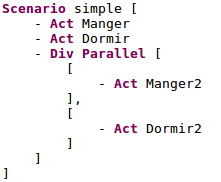
\includegraphics[]{figures/xtext.png}
%		\caption{Exemple de syntaxe textuelle avec Xtext}
%		\label{Xtext}
%	\end{center}
%\end{figure}

\end{document}